\documentclass[12pt]{article}
\usepackage{amsmath}
\usepackage{amssymb}
\usepackage{amsfonts}
\usepackage[colorlinks=true]{hyperref}
\usepackage{graphicx}

\title{Prvi Doma\'{c}i zadatak}
\author{TZS}
\date{\today}

\begin{document}
\maketitle

U izradi doma\'{c}eg zadatka se mo\v{z}ete konsultovati medjusobno i sa mnom. Svaki doma\'{c}i koji predajete, medjutim, mora biti samostalno napisan. 

\textbf{Rok za predaju ovog doma\'{c}eg zadatka je petak 18.11.2022. Prvi i drugi zadatak nose po 8 poena a tre\'{c}i 4 poena.}

\section*{Zadatak 1}

Razmatrajmo polubeskona\v{c}nu, plan-paralelnu atmosferu u kojoj funkcija izvora na nekoj, referentnoj talasnoj du\v{z}ini zavisi od opti\v{c}ke dubine kao:
\begin{equation}
S = a + b\tau
\end{equation}
Ovo je poznato kao Milne-Eddingtonova (ili Milne-Barbier-Unsold approksimacija) i na osnovu nje mozemo da dodjemo do raznih korisnih relacija koje nam omogu\'{c}avaju da bolje razumemo zvezdane atmosfere. Medjutim, u zvezdanim atmosferama bi imalo vi\v{s}e smisla koristiti $\ln \tau$ kao skalu dubine. Pretpostavimo, dakle, da na\v{s}a funkcija izvora zavisi od referentne opti\v{c}ke dubine kao:
\begin{equation}
S = a + b\ln\tau
\end{equation}


\begin{itemize}
    \item Re\v{s}iti jedna{v}cinu prenosa zra\v{c}enja na referentnoj talasnoj du\v{z}ini, tj. izraziti izlazni intenzitet preko konstanti $a, b$. Ovaj intenzitet \'{c}emo zvati $I^+$. Napomena: Integral koji se dobija nije mogu\'{c}e re\v{s}iti analiti\v{c}ki, tako da morate iskoristiti npr. Mathematicu, Wolfram Alpha ili sli\v{c}no.
    
    \item Ova pretpostavka ima jedan konceptualan problem a to je da na malim opti\v{c}kim dubinama, $\ln \tau$ ide u $-\infty$ pa, bez obzira koliko je koeficijent $b$ mali, funkcija izvora bi postala negativna. To mo\v{z}emo da popravimo tako \v{s}to \'{c}emo pretpostaviti da je funkcija izvora paraboli\v{c}na funkcija od $\ln \tau$:
    \begin{equation}
        S = a + b\ln \tau + c \ln^2 \tau
    \end{equation}
    Re\v{s}iti jedna\v{c}inu prenosa za ovakav oblik funkcije izvora. 
    
    \item Pretpostavimo (va\v{z}i za relativno velike talasne du\v{z}ine) da je funkcija izvora propoprcionalna Temperaturi. Jednostavnosti radi uzmimo da je konstanta proporcionalnosti jednaka jedan. Na\'{c}i $a, b, c$ tako da je $T(\ln\tau=0) = 6000$ (fotosfera), $T(\ln\tau=-7) = 4500$ (tzv. temperaturski minimum), $T(\ln\tau=-14) = 8000$ (hromosfera). Izra\v{c}unaj numeri\v{c}ku vrednost $I^+$. Da li va\v{z}i da je izlazni intenzitet pribli\v{z}no jednak funkciji izvora na $\tau=1$?

    \item Kakav bi bio izlazni intenzitet na talasnoj du\v{z}ini na kojoj je koeficijent neprozra\v{c}nosti $r_\lambda$ puta ve\'{c}i od referentnog? Skicirajte / isplotujte zavisnost $I^+_\lambda$ od $r_\lambda$ ($r_\lambda >  1$).
    
\end{itemize}

\section*{Zadatak 2}

Tipi\v{c}na temperatura u sun\v{c}evoj fotosferi je 6000K a ukupan pritisak gasa oko $10^5 {\rm dyn/cm^2}$ \v{s}to je oko 1\,Pa. Pod pretpostavkom da je fotosfera u potpunosti sa\v{c}injena od vodonika, proceni:
\begin{itemize}
    \item Koncentraciju pozitivno naelektrisanih jona vodonika (protona), i koncentraciju elektrona.
    \item Koncentraciju negativno naelektrisanih jona vodonika. Za ovaj deo mo\v{z}ete pretpostaviti da je najve\'{c}i deo atoma vodonika neutralan. Energija jonizacije H$^-$ jona je 0.75\,eV.
    \item Uporedite koncentraciju negativno naelektrisanog jona vodonika sa koncentracijama atoma vodonika ekscitovanih na $n=3$ i $n=2$.
    \item \v{S}ta nam ovo govori o va\v{z}nosti Balmerovog, odnosno Pa\v{s}enovog kontinuuma sa apsorpciju u Sun\v{c}evoj fotosferi, u odnosu na negativan jon vodonika?
\end{itemize}

\section*{Zadatak 3}

Protuberance (eng: \emph{prominences}) i filamenti su po na\v{s}em trenutnom shvatanju jedni te isti objekti (videti sliku): relativno hladne koncentracije gasa koje pod uticajem magnetnog polja ``vise'' u Sun\v{c}evoj koroni. Filamente vidimo na disku: nevidljivi su u kontinuumu, ali se vide kao tamne ``trake'' na talasnim du\v{z}inama u centru jakih spektralnih linija (npr. H$\alpha$). Protuberance, sa druge strane, se vide iznad Sun\v{c}evog ruba kao svetle formacije u centru jakih spektralnih linija. Ukoliko su posmatra\v{c}ki uslovi izuzetni, mogu se videti i u kontinuumu. Koriste\'{c}i formalizam prenosa zra\v{c}enja, objasniti razliku izmedju protuberanci i filamenata.

\begin{figure}
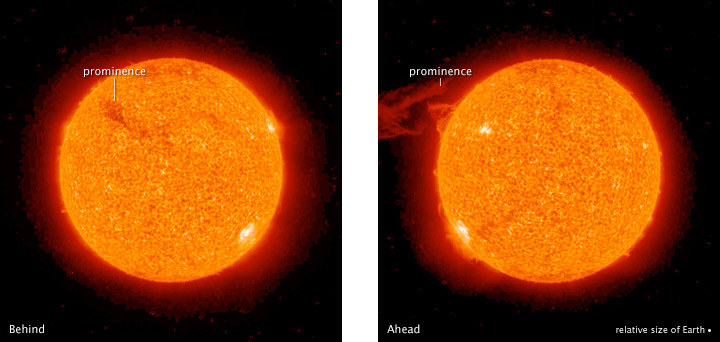
\includegraphics[width=\textwidth]{prominence.jpg}
\caption{Levo: primer sun\v{c}evog filamenta. Desno: Isti taj filament, koji se vidi kao protuberanca.}
\end{figure}




\end{document}
